\documentclass[11pt,oneside, a4paper]{amsart}\usepackage[]{graphicx}\usepackage[]{color}
%% maxwidth is the original width if it is less than linewidth
%% otherwise use linewidth (to make sure the graphics do not exceed the margin)
\makeatletter
\def\maxwidth{ %
  \ifdim\Gin@nat@width>\linewidth
    \linewidth
  \else
    \Gin@nat@width
  \fi
}
\makeatother

\definecolor{fgcolor}{rgb}{0.345, 0.345, 0.345}
\newcommand{\hlnum}[1]{\textcolor[rgb]{0.686,0.059,0.569}{#1}}%
\newcommand{\hlstr}[1]{\textcolor[rgb]{0.192,0.494,0.8}{#1}}%
\newcommand{\hlcom}[1]{\textcolor[rgb]{0.678,0.584,0.686}{\textit{#1}}}%
\newcommand{\hlopt}[1]{\textcolor[rgb]{0,0,0}{#1}}%
\newcommand{\hlstd}[1]{\textcolor[rgb]{0.345,0.345,0.345}{#1}}%
\newcommand{\hlkwa}[1]{\textcolor[rgb]{0.161,0.373,0.58}{\textbf{#1}}}%
\newcommand{\hlkwb}[1]{\textcolor[rgb]{0.69,0.353,0.396}{#1}}%
\newcommand{\hlkwc}[1]{\textcolor[rgb]{0.333,0.667,0.333}{#1}}%
\newcommand{\hlkwd}[1]{\textcolor[rgb]{0.737,0.353,0.396}{\textbf{#1}}}%

\usepackage{framed}
\makeatletter
\newenvironment{kframe}{%
 \def\at@end@of@kframe{}%
 \ifinner\ifhmode%
  \def\at@end@of@kframe{\end{minipage}}%
  \begin{minipage}{\columnwidth}%
 \fi\fi%
 \def\FrameCommand##1{\hskip\@totalleftmargin \hskip-\fboxsep
 \colorbox{shadecolor}{##1}\hskip-\fboxsep
     % There is no \\@totalrightmargin, so:
     \hskip-\linewidth \hskip-\@totalleftmargin \hskip\columnwidth}%
 \MakeFramed {\advance\hsize-\width
   \@totalleftmargin\z@ \linewidth\hsize
   \@setminipage}}%
 {\par\unskip\endMakeFramed%
 \at@end@of@kframe}
\makeatother

\definecolor{shadecolor}{rgb}{.97, .97, .97}
\definecolor{messagecolor}{rgb}{0, 0, 0}
\definecolor{warningcolor}{rgb}{1, 0, 1}
\definecolor{errorcolor}{rgb}{1, 0, 0}
\newenvironment{knitrout}{}{} % an empty environment to be redefined in TeX

\usepackage{alltt}
\usepackage{natbib}

\usepackage{amsbsy,amsmath}
\usepackage{amssymb,amsfonts}
\usepackage{bbm}%give 1 with dbl vertical bar 
\usepackage{booktabs,url,enumerate}
\usepackage{color,xcolor,colortbl}
\usepackage{float}
\usepackage{tikz}
\usepackage{rotating,graphicx,lscape}
\usepackage{commath}
\usetikzlibrary{arrows,positioning} 
\usepackage[hypcap]{caption}
\newcommand{\sgn}{\mathrm{sign}}
\usepackage{setspace}

% bold rows
\usepackage{array}
\newcolumntype{$}{>{\global\let\currentrowstyle\relax}}
\newcolumntype{^}{>{\currentrowstyle}}
\newcommand{\rowstyle}[1]{\gdef\currentrowstyle{#1}%
  #1\ignorespaces
}

% Invisible table columns!
\newcolumntype{H}{>{\setbox0=\hbox\bgroup}c<{\egroup}@{}}% Properly placed sideways table with asmart class. 

\setlength\rotFPtop{0pt plus 1fil} 


\usepackage[top=1.5cm, bottom=1.5cm, left=3.0cm, right=3.0cm]{geometry}

\DeclareMathOperator{\Med}{\mathbb{M}ed}
\DeclareMathOperator{\Mean}{\mathbb{M}ean}
\DeclareMathOperator{\Cov}{\mathbb{C}ov}
\DeclareMathOperator{\Var}{\mathbb{V}ar}
\DeclareMathOperator{\E}{\mathbb{E}}
\DeclareMathOperator{\nid}{NID}
\DeclareMathOperator{\N}{\mathcal{N}}
\DeclareMathOperator{\corr}{corr}
\DeclareMathOperator{\diag}{diag}
\onehalfspace


\definecolor{LightRed}{rgb}{1,.88,.88}
\definecolor{LightBlue}{rgb}{.88,.88,1}
\definecolor{LightGreen}{rgb}{.88,1,.88}

\newtheorem{theorem}{Theorem}
\IfFileExists{upquote.sty}{\usepackage{upquote}}{}
\begin{document}

  
\title{IRF}   
\author{Clément Carrier}
\date{\today}
\maketitle


\section*{Forecast performance}

In this section, using a sample from Q1 1998 to Q4 2009, I forecast HICP from Q1 2010 to Q4 2013 with several models. These models difer thanks to the number of lag used, if they are adaptive or not. \\

I plot the results and give the RMSE of these forecasts. \\

Here is the R code : 


\begin{knitrout}
\definecolor{shadecolor}{rgb}{0.969, 0.969, 0.969}\color{fgcolor}\begin{kframe}
\begin{alltt}
\hlkwd{library}\hlstd{(knitr); opts_chunk}\hlopt{$}\hlkwd{set}\hlstd{(}\hlkwc{message}\hlstd{=}\hlnum{FALSE}\hlstd{)}
\end{alltt}
\end{kframe}
\end{knitrout}

\begin{knitrout}
\definecolor{shadecolor}{rgb}{0.969, 0.969, 0.969}\color{fgcolor}\begin{kframe}
\begin{alltt}
\hlkwd{require}\hlstd{(lassovar)}
\hlkwd{require}\hlstd{(ggplot2)}
\hlkwd{require}\hlstd{(reshape2)}
\hlkwd{require}\hlstd{(urca)}
\hlkwd{require}\hlstd{(MSBVAR)}
\hlkwd{library}\hlstd{(xtable)}
\end{alltt}
\end{kframe}
\end{knitrout}


\begin{knitrout}
\definecolor{shadecolor}{rgb}{0.969, 0.969, 0.969}\color{fgcolor}\begin{kframe}
\begin{alltt}
\hlstd{forecast2}\hlkwb{<-}\hlkwa{function}\hlstd{(}\hlkwc{data}\hlstd{,}\hlkwc{lag}\hlstd{,}\hlkwc{horizon}\hlstd{,}\hlkwc{preforecast}\hlstd{)\{}
  \hlstd{fore}\hlkwb{<-}\hlkwd{matrix}\hlstd{(}\hlnum{0}\hlstd{,}\hlkwc{nrow}\hlstd{=}\hlkwd{dim}\hlstd{(data)[}\hlnum{2}\hlstd{],}\hlkwc{ncol}\hlstd{=horizon}\hlopt{+}\hlstd{preforecast)}
  \hlstd{fore[,}\hlnum{1}\hlopt{:}\hlstd{(preforecast)]}\hlkwb{<-}\hlkwd{t}\hlstd{(data[(}\hlkwd{dim}\hlstd{(data)[}\hlnum{1}\hlstd{]}\hlopt{-}\hlstd{preforecast}\hlopt{+}\hlnum{1}\hlstd{)}\hlopt{:}\hlkwd{dim}\hlstd{(data)[}\hlnum{1}\hlstd{],])}
  \hlstd{lv}\hlkwb{<-}\hlkwd{lassovar}\hlstd{(}\hlkwc{dat}\hlstd{=data,}\hlkwc{lags}\hlstd{=lag)}
  \hlstd{intercept}\hlkwb{<-}\hlkwd{as.matrix}\hlstd{(lv}\hlopt{$}\hlstd{coefficients[}\hlnum{1}\hlstd{,],}\hlkwd{dim}\hlstd{(data)[}\hlnum{2}\hlstd{],}\hlnum{1}\hlstd{)}
  \hlkwa{if}\hlstd{(lag}\hlopt{==}\hlnum{1}\hlstd{)\{}
    \hlstd{coeff}\hlkwb{<-}\hlkwd{as.matrix}\hlstd{(}\hlkwd{t}\hlstd{(lv}\hlopt{$}\hlstd{coefficients[}\hlopt{-}\hlnum{1}\hlstd{,]),}\hlkwd{dim}\hlstd{(data)[}\hlnum{2}\hlstd{],}\hlkwd{dim}\hlstd{(data)[}\hlnum{2}\hlstd{])}
    \hlkwa{for} \hlstd{(i} \hlkwa{in} \hlstd{(preforecast}\hlopt{+}\hlnum{1}\hlstd{)}\hlopt{:}\hlstd{(horizon}\hlopt{+}\hlstd{preforecast))\{}
      \hlstd{fore[,i]}\hlkwb{<-}\hlstd{intercept}\hlopt{+}\hlstd{coeff}\hlopt\hlstd{fore[,i}\hlopt{-}\hlnum{1}\hlstd{]}
    \hlstd{\}}
  \hlstd{\}} \hlkwa{else} \hlstd{\{}
    \hlkwa{if}\hlstd{(lag}\hlopt{==}\hlnum{2}\hlstd{)\{}
      \hlstd{coeff1}\hlkwb{<-}\hlkwd{as.matrix}\hlstd{(}\hlkwd{t}\hlstd{(lv}\hlopt{$}\hlstd{coefficients[}\hlnum{2}\hlopt{:}\hlstd{(}\hlkwd{dim}\hlstd{(data)[}\hlnum{2}\hlstd{]}\hlopt{+}\hlnum{1}\hlstd{),]),}
                        \hlkwd{dim}\hlstd{(data)[}\hlnum{2}\hlstd{],}\hlkwd{dim}\hlstd{(data)[}\hlnum{2}\hlstd{])}
      \hlstd{coeff2}\hlkwb{<-}\hlkwd{as.matrix}\hlstd{(}\hlkwd{t}\hlstd{(lv}\hlopt{$}\hlstd{coefficients[(}\hlkwd{dim}\hlstd{(data)[}\hlnum{2}\hlstd{]}\hlopt{+}\hlnum{2}\hlstd{)}\hlopt{:}\hlstd{(}\hlnum{2}\hlopt{*}\hlkwd{dim}\hlstd{(data)[}\hlnum{2}\hlstd{]}\hlopt{+}\hlnum{1}\hlstd{),]),}
                        \hlkwd{dim}\hlstd{(data)[}\hlnum{2}\hlstd{],}\hlkwd{dim}\hlstd{(data)[}\hlnum{2}\hlstd{])}
      \hlkwa{for} \hlstd{(i} \hlkwa{in} \hlstd{(preforecast}\hlopt{+}\hlnum{1}\hlstd{)}\hlopt{:}\hlstd{(horizon}\hlopt{+}\hlstd{preforecast))\{}
        \hlstd{fore[,i]}\hlkwb{<-}\hlstd{intercept}\hlopt{+}\hlstd{coeff1}\hlopt\hlstd{fore[,i}\hlopt{-}\hlnum{1}\hlstd{]}\hlopt{+}\hlstd{coeff2}\hlopt\hlstd{fore[,i}\hlopt{-}\hlnum{2}\hlstd{]}
      \hlstd{\}}
    \hlstd{\}} \hlkwa{else} \hlstd{\{}
      \hlkwa{if}\hlstd{(lag}\hlopt{==}\hlnum{3}\hlstd{)\{}
        \hlstd{coeff1}\hlkwb{<-}\hlkwd{as.matrix}\hlstd{(}\hlkwd{t}\hlstd{(lv}\hlopt{$}\hlstd{coefficients[}\hlnum{2}\hlopt{:}\hlstd{(}\hlkwd{dim}\hlstd{(data)[}\hlnum{2}\hlstd{]}\hlopt{+}\hlnum{1}\hlstd{),]),}
                          \hlkwd{dim}\hlstd{(data)[}\hlnum{2}\hlstd{],}\hlkwd{dim}\hlstd{(data)[}\hlnum{2}\hlstd{])}
        \hlstd{coeff2}\hlkwb{<-}\hlkwd{as.matrix}\hlstd{(}\hlkwd{t}\hlstd{(lv}\hlopt{$}\hlstd{coefficients[(}\hlkwd{dim}\hlstd{(data)[}\hlnum{2}\hlstd{]}\hlopt{+}\hlnum{2}\hlstd{)}\hlopt{:}\hlstd{(}\hlnum{2}\hlopt{*}\hlkwd{dim}\hlstd{(data)[}\hlnum{2}\hlstd{]}\hlopt{+}\hlnum{1}\hlstd{),]),}
                          \hlkwd{dim}\hlstd{(data)[}\hlnum{2}\hlstd{],}\hlkwd{dim}\hlstd{(data)[}\hlnum{2}\hlstd{])}
        \hlstd{coeff3}\hlkwb{<-}\hlkwd{as.matrix}\hlstd{(}\hlkwd{t}\hlstd{(lv}\hlopt{$}\hlstd{coefficients[(}\hlnum{2}\hlopt{*}\hlkwd{dim}\hlstd{(data)[}\hlnum{2}\hlstd{]}\hlopt{+}\hlnum{2}\hlstd{)}\hlopt{:}\hlstd{(}\hlnum{3}\hlopt{*}\hlkwd{dim}\hlstd{(data)[}\hlnum{2}\hlstd{]}\hlopt{+}\hlnum{1}\hlstd{),]),}
                          \hlkwd{dim}\hlstd{(data)[}\hlnum{2}\hlstd{],}\hlkwd{dim}\hlstd{(data)[}\hlnum{2}\hlstd{])}
        \hlkwa{for} \hlstd{(i} \hlkwa{in} \hlstd{(preforecast}\hlopt{+}\hlnum{1}\hlstd{)}\hlopt{:}\hlstd{(horizon}\hlopt{+}\hlstd{preforecast))\{}
          \hlstd{fore[,i]}\hlkwb{<-}\hlstd{intercept}\hlopt{+}\hlstd{coeff1}\hlopt\hlstd{fore[,i}\hlopt{-}\hlnum{1}\hlstd{]}\hlopt{+}\hlstd{coeff2}\hlopt\hlstd{fore[,i}\hlopt{-}\hlnum{2}\hlstd{]}\hlopt{+}
            \hlstd{coeff3}\hlopt\hlstd{fore[,i}\hlopt{-}\hlnum{3}\hlstd{]}
        \hlstd{\}}
      \hlstd{\}}
      \hlkwa{else} \hlstd{\{}
        \hlstd{coeff1}\hlkwb{<-}\hlkwd{as.matrix}\hlstd{(}\hlkwd{t}\hlstd{(lv}\hlopt{$}\hlstd{coefficients[}\hlnum{2}\hlopt{:}\hlstd{(}\hlkwd{dim}\hlstd{(data)[}\hlnum{2}\hlstd{]}\hlopt{+}\hlnum{1}\hlstd{),]),}
                          \hlkwd{dim}\hlstd{(data)[}\hlnum{2}\hlstd{],}\hlkwd{dim}\hlstd{(data)[}\hlnum{2}\hlstd{])}
        \hlstd{coeff2}\hlkwb{<-}\hlkwd{as.matrix}\hlstd{(}\hlkwd{t}\hlstd{(lv}\hlopt{$}\hlstd{coefficients[(}\hlkwd{dim}\hlstd{(data)[}\hlnum{2}\hlstd{]}\hlopt{+}\hlnum{2}\hlstd{)}\hlopt{:}\hlstd{(}\hlnum{2}\hlopt{*}\hlkwd{dim}\hlstd{(data)[}\hlnum{2}\hlstd{]}\hlopt{+}\hlnum{1}\hlstd{),]),}
                          \hlkwd{dim}\hlstd{(data)[}\hlnum{2}\hlstd{],}\hlkwd{dim}\hlstd{(data)[}\hlnum{2}\hlstd{])}
        \hlstd{coeff3}\hlkwb{<-}\hlkwd{as.matrix}\hlstd{(}\hlkwd{t}\hlstd{(lv}\hlopt{$}\hlstd{coefficients[(}\hlnum{2}\hlopt{*}\hlkwd{dim}\hlstd{(data)[}\hlnum{2}\hlstd{]}\hlopt{+}\hlnum{2}\hlstd{)}\hlopt{:}\hlstd{(}\hlnum{3}\hlopt{*}\hlkwd{dim}\hlstd{(data)[}\hlnum{2}\hlstd{]}\hlopt{+}\hlnum{1}\hlstd{),]),}
                          \hlkwd{dim}\hlstd{(data)[}\hlnum{2}\hlstd{],}\hlkwd{dim}\hlstd{(data)[}\hlnum{2}\hlstd{])}
        \hlstd{coeff4}\hlkwb{<-}\hlkwd{as.matrix}\hlstd{(}\hlkwd{t}\hlstd{(lv}\hlopt{$}\hlstd{coefficients[(}\hlnum{3}\hlopt{*}\hlkwd{dim}\hlstd{(data)[}\hlnum{2}\hlstd{]}\hlopt{+}\hlnum{2}\hlstd{)}\hlopt{:}\hlstd{(}\hlnum{4}\hlopt{*}\hlkwd{dim}\hlstd{(data)[}\hlnum{2}\hlstd{]}\hlopt{+}\hlnum{1}\hlstd{),]),}
                          \hlkwd{dim}\hlstd{(data)[}\hlnum{2}\hlstd{],}\hlkwd{dim}\hlstd{(data)[}\hlnum{2}\hlstd{])}
        \hlkwa{for} \hlstd{(i} \hlkwa{in} \hlstd{(preforecast}\hlopt{+}\hlnum{1}\hlstd{)}\hlopt{:}\hlstd{(horizon}\hlopt{+}\hlstd{preforecast))\{}
          \hlstd{fore[,i]}\hlkwb{<-}\hlstd{intercept}\hlopt{+}\hlstd{coeff1}\hlopt\hlstd{fore[,i}\hlopt{-}\hlnum{1}\hlstd{]}\hlopt{+}\hlstd{coeff2}\hlopt\hlstd{fore[,i}\hlopt{-}\hlnum{2}\hlstd{]}\hlopt{+}
            \hlstd{coeff3}\hlopt\hlstd{fore[,i}\hlopt{-}\hlnum{3}\hlstd{]}\hlopt{+}\hlstd{coeff4}\hlopt\hlstd{fore[,i}\hlopt{-}\hlnum{4}\hlstd{]}
        \hlstd{\}}
      \hlstd{\}}
    \hlstd{\}}
  \hlstd{\}}
  \hlkwd{rownames}\hlstd{(fore)}\hlkwb{<-}\hlkwd{names}\hlstd{(data)}
  \hlkwd{return}\hlstd{(}\hlkwd{t}\hlstd{(fore))}
\hlstd{\}}



\hlstd{forecast2adaptlasso}\hlkwb{<-}\hlkwa{function}\hlstd{(}\hlkwc{data}\hlstd{,}\hlkwc{lag}\hlstd{,}\hlkwc{horizon}\hlstd{,}\hlkwc{preforecast}\hlstd{)\{}
  \hlstd{fore}\hlkwb{<-}\hlkwd{matrix}\hlstd{(}\hlnum{0}\hlstd{,}\hlkwc{nrow}\hlstd{=}\hlkwd{dim}\hlstd{(data)[}\hlnum{2}\hlstd{],}\hlkwc{ncol}\hlstd{=horizon}\hlopt{+}\hlstd{preforecast)}
  \hlstd{fore[,}\hlnum{1}\hlopt{:}\hlstd{(preforecast)]}\hlkwb{<-}\hlkwd{t}\hlstd{(data[(}\hlkwd{dim}\hlstd{(data)[}\hlnum{1}\hlstd{]}\hlopt{-}\hlstd{preforecast}\hlopt{+}\hlnum{1}\hlstd{)}\hlopt{:}\hlkwd{dim}\hlstd{(data)[}\hlnum{1}\hlstd{],])}
  \hlstd{lv}\hlkwb{<-}\hlkwd{lassovar}\hlstd{(}\hlkwc{dat}\hlstd{=data,}\hlkwc{lags}\hlstd{=lag,}\hlkwc{adaptive}\hlstd{=}\hlstr{'lasso'}\hlstd{)}
  \hlstd{intercept}\hlkwb{<-}\hlkwd{as.matrix}\hlstd{(lv}\hlopt{$}\hlstd{coefficients[}\hlnum{1}\hlstd{,],}\hlkwd{dim}\hlstd{(data)[}\hlnum{2}\hlstd{],}\hlnum{1}\hlstd{)}
  \hlkwa{if}\hlstd{(lag}\hlopt{==}\hlnum{1}\hlstd{)\{}
    \hlstd{coeff}\hlkwb{<-}\hlkwd{as.matrix}\hlstd{(}\hlkwd{t}\hlstd{(lv}\hlopt{$}\hlstd{coefficients[}\hlopt{-}\hlnum{1}\hlstd{,]),}\hlkwd{dim}\hlstd{(data)[}\hlnum{2}\hlstd{],}\hlkwd{dim}\hlstd{(data)[}\hlnum{2}\hlstd{])}
    \hlkwa{for} \hlstd{(i} \hlkwa{in} \hlstd{(preforecast}\hlopt{+}\hlnum{1}\hlstd{)}\hlopt{:}\hlstd{(horizon}\hlopt{+}\hlstd{preforecast))\{}
      \hlstd{fore[,i]}\hlkwb{<-}\hlstd{intercept}\hlopt{+}\hlstd{coeff}\hlopt\hlstd{fore[,i}\hlopt{-}\hlnum{1}\hlstd{]}
    \hlstd{\}}
  \hlstd{\}} \hlkwa{else} \hlstd{\{}
    \hlkwa{if}\hlstd{(lag}\hlopt{==}\hlnum{2}\hlstd{)\{}
      \hlstd{coeff1}\hlkwb{<-}\hlkwd{as.matrix}\hlstd{(}\hlkwd{t}\hlstd{(lv}\hlopt{$}\hlstd{coefficients[}\hlnum{2}\hlopt{:}\hlstd{(}\hlkwd{dim}\hlstd{(data)[}\hlnum{2}\hlstd{]}\hlopt{+}\hlnum{1}\hlstd{),]),}
                        \hlkwd{dim}\hlstd{(data)[}\hlnum{2}\hlstd{],}\hlkwd{dim}\hlstd{(data)[}\hlnum{2}\hlstd{])}
      \hlstd{coeff2}\hlkwb{<-}\hlkwd{as.matrix}\hlstd{(}\hlkwd{t}\hlstd{(lv}\hlopt{$}\hlstd{coefficients[(}\hlkwd{dim}\hlstd{(data)[}\hlnum{2}\hlstd{]}\hlopt{+}\hlnum{2}\hlstd{)}\hlopt{:}\hlstd{(}\hlnum{2}\hlopt{*}\hlkwd{dim}\hlstd{(data)[}\hlnum{2}\hlstd{]}\hlopt{+}\hlnum{1}\hlstd{),]),}
                        \hlkwd{dim}\hlstd{(data)[}\hlnum{2}\hlstd{],}\hlkwd{dim}\hlstd{(data)[}\hlnum{2}\hlstd{])}
      \hlkwa{for} \hlstd{(i} \hlkwa{in} \hlstd{(preforecast}\hlopt{+}\hlnum{1}\hlstd{)}\hlopt{:}\hlstd{(horizon}\hlopt{+}\hlstd{preforecast))\{}
        \hlstd{fore[,i]}\hlkwb{<-}\hlstd{intercept}\hlopt{+}\hlstd{coeff1}\hlopt\hlstd{fore[,i}\hlopt{-}\hlnum{1}\hlstd{]}\hlopt{+}\hlstd{coeff2}\hlopt\hlstd{fore[,i}\hlopt{-}\hlnum{2}\hlstd{]}
      \hlstd{\}}
    \hlstd{\}} \hlkwa{else} \hlstd{\{}
      \hlkwa{if}\hlstd{(lag}\hlopt{==}\hlnum{3}\hlstd{)\{}
        \hlstd{coeff1}\hlkwb{<-}\hlkwd{as.matrix}\hlstd{(}\hlkwd{t}\hlstd{(lv}\hlopt{$}\hlstd{coefficients[}\hlnum{2}\hlopt{:}\hlstd{(}\hlkwd{dim}\hlstd{(data)[}\hlnum{2}\hlstd{]}\hlopt{+}\hlnum{1}\hlstd{),]),}
                          \hlkwd{dim}\hlstd{(data)[}\hlnum{2}\hlstd{],}\hlkwd{dim}\hlstd{(data)[}\hlnum{2}\hlstd{])}
        \hlstd{coeff2}\hlkwb{<-}\hlkwd{as.matrix}\hlstd{(}\hlkwd{t}\hlstd{(lv}\hlopt{$}\hlstd{coefficients[(}\hlkwd{dim}\hlstd{(data)[}\hlnum{2}\hlstd{]}\hlopt{+}\hlnum{2}\hlstd{)}\hlopt{:}\hlstd{(}\hlnum{2}\hlopt{*}\hlkwd{dim}\hlstd{(data)[}\hlnum{2}\hlstd{]}\hlopt{+}\hlnum{1}\hlstd{),]),}
                          \hlkwd{dim}\hlstd{(data)[}\hlnum{2}\hlstd{],}\hlkwd{dim}\hlstd{(data)[}\hlnum{2}\hlstd{])}
        \hlstd{coeff3}\hlkwb{<-}\hlkwd{as.matrix}\hlstd{(}\hlkwd{t}\hlstd{(lv}\hlopt{$}\hlstd{coefficients[(}\hlnum{2}\hlopt{*}\hlkwd{dim}\hlstd{(data)[}\hlnum{2}\hlstd{]}\hlopt{+}\hlnum{2}\hlstd{)}\hlopt{:}\hlstd{(}\hlnum{3}\hlopt{*}\hlkwd{dim}\hlstd{(data)[}\hlnum{2}\hlstd{]}\hlopt{+}\hlnum{1}\hlstd{),]),}
                          \hlkwd{dim}\hlstd{(data)[}\hlnum{2}\hlstd{],}\hlkwd{dim}\hlstd{(data)[}\hlnum{2}\hlstd{])}
        \hlkwa{for} \hlstd{(i} \hlkwa{in} \hlstd{(preforecast}\hlopt{+}\hlnum{1}\hlstd{)}\hlopt{:}\hlstd{(horizon}\hlopt{+}\hlstd{preforecast))\{}
          \hlstd{fore[,i]}\hlkwb{<-}\hlstd{intercept}\hlopt{+}\hlstd{coeff1}\hlopt\hlstd{fore[,i}\hlopt{-}\hlnum{1}\hlstd{]}\hlopt{+}\hlstd{coeff2}\hlopt\hlstd{fore[,i}\hlopt{-}\hlnum{2}\hlstd{]}\hlopt{+}
            \hlstd{coeff3}\hlopt\hlstd{fore[,i}\hlopt{-}\hlnum{3}\hlstd{]}
        \hlstd{\}}
      \hlstd{\}}
      \hlkwa{else} \hlstd{\{}
        \hlstd{coeff1}\hlkwb{<-}\hlkwd{as.matrix}\hlstd{(}\hlkwd{t}\hlstd{(lv}\hlopt{$}\hlstd{coefficients[}\hlnum{2}\hlopt{:}\hlstd{(}\hlkwd{dim}\hlstd{(data)[}\hlnum{2}\hlstd{]}\hlopt{+}\hlnum{1}\hlstd{),]),}
                          \hlkwd{dim}\hlstd{(data)[}\hlnum{2}\hlstd{],}\hlkwd{dim}\hlstd{(data)[}\hlnum{2}\hlstd{])}
        \hlstd{coeff2}\hlkwb{<-}\hlkwd{as.matrix}\hlstd{(}\hlkwd{t}\hlstd{(lv}\hlopt{$}\hlstd{coefficients[(}\hlkwd{dim}\hlstd{(data)[}\hlnum{2}\hlstd{]}\hlopt{+}\hlnum{2}\hlstd{)}\hlopt{:}\hlstd{(}\hlnum{2}\hlopt{*}\hlkwd{dim}\hlstd{(data)[}\hlnum{2}\hlstd{]}\hlopt{+}\hlnum{1}\hlstd{),]),}
                          \hlkwd{dim}\hlstd{(data)[}\hlnum{2}\hlstd{],}\hlkwd{dim}\hlstd{(data)[}\hlnum{2}\hlstd{])}
        \hlstd{coeff3}\hlkwb{<-}\hlkwd{as.matrix}\hlstd{(}\hlkwd{t}\hlstd{(lv}\hlopt{$}\hlstd{coefficients[(}\hlnum{2}\hlopt{*}\hlkwd{dim}\hlstd{(data)[}\hlnum{2}\hlstd{]}\hlopt{+}\hlnum{2}\hlstd{)}\hlopt{:}\hlstd{(}\hlnum{3}\hlopt{*}\hlkwd{dim}\hlstd{(data)[}\hlnum{2}\hlstd{]}\hlopt{+}\hlnum{1}\hlstd{),]),}
                          \hlkwd{dim}\hlstd{(data)[}\hlnum{2}\hlstd{],}\hlkwd{dim}\hlstd{(data)[}\hlnum{2}\hlstd{])}
        \hlstd{coeff4}\hlkwb{<-}\hlkwd{as.matrix}\hlstd{(}\hlkwd{t}\hlstd{(lv}\hlopt{$}\hlstd{coefficients[(}\hlnum{3}\hlopt{*}\hlkwd{dim}\hlstd{(data)[}\hlnum{2}\hlstd{]}\hlopt{+}\hlnum{2}\hlstd{)}\hlopt{:}\hlstd{(}\hlnum{4}\hlopt{*}\hlkwd{dim}\hlstd{(data)[}\hlnum{2}\hlstd{]}\hlopt{+}\hlnum{1}\hlstd{),]),}
                          \hlkwd{dim}\hlstd{(data)[}\hlnum{2}\hlstd{],}\hlkwd{dim}\hlstd{(data)[}\hlnum{2}\hlstd{])}
        \hlkwa{for} \hlstd{(i} \hlkwa{in} \hlstd{(preforecast}\hlopt{+}\hlnum{1}\hlstd{)}\hlopt{:}\hlstd{(horizon}\hlopt{+}\hlstd{preforecast))\{}
          \hlstd{fore[,i]}\hlkwb{<-}\hlstd{intercept}\hlopt{+}\hlstd{coeff1}\hlopt\hlstd{fore[,i}\hlopt{-}\hlnum{1}\hlstd{]}\hlopt{+}\hlstd{coeff2}\hlopt\hlstd{fore[,i}\hlopt{-}\hlnum{2}\hlstd{]}\hlopt{+}
            \hlstd{coeff3}\hlopt\hlstd{fore[,i}\hlopt{-}\hlnum{3}\hlstd{]}\hlopt{+}\hlstd{coeff4}\hlopt\hlstd{fore[,i}\hlopt{-}\hlnum{4}\hlstd{]}
        \hlstd{\}}
      \hlstd{\}}
    \hlstd{\}}
  \hlstd{\}}
  \hlkwd{rownames}\hlstd{(fore)}\hlkwb{<-}\hlkwd{names}\hlstd{(data)}
  \hlkwd{return}\hlstd{(}\hlkwd{t}\hlstd{(fore))}
\hlstd{\}}

\hlstd{forecast2adaptridge}\hlkwb{<-}\hlkwa{function}\hlstd{(}\hlkwc{data}\hlstd{,}\hlkwc{lag}\hlstd{,}\hlkwc{horizon}\hlstd{,}\hlkwc{preforecast}\hlstd{)\{}
  \hlstd{fore}\hlkwb{<-}\hlkwd{matrix}\hlstd{(}\hlnum{0}\hlstd{,}\hlkwc{nrow}\hlstd{=}\hlkwd{dim}\hlstd{(data)[}\hlnum{2}\hlstd{],}\hlkwc{ncol}\hlstd{=horizon}\hlopt{+}\hlstd{preforecast)}
  \hlstd{fore[,}\hlnum{1}\hlopt{:}\hlstd{(preforecast)]}\hlkwb{<-}\hlkwd{t}\hlstd{(data[(}\hlkwd{dim}\hlstd{(data)[}\hlnum{1}\hlstd{]}\hlopt{-}\hlstd{preforecast}\hlopt{+}\hlnum{1}\hlstd{)}\hlopt{:}\hlkwd{dim}\hlstd{(data)[}\hlnum{1}\hlstd{],])}
  \hlstd{lv}\hlkwb{<-}\hlkwd{lassovar}\hlstd{(}\hlkwc{dat}\hlstd{=data,}\hlkwc{lags}\hlstd{=lag,}\hlkwc{adaptive}\hlstd{=}\hlstr{'ridge'}\hlstd{)}
  \hlstd{intercept}\hlkwb{<-}\hlkwd{as.matrix}\hlstd{(lv}\hlopt{$}\hlstd{coefficients[}\hlnum{1}\hlstd{,],}\hlkwd{dim}\hlstd{(data)[}\hlnum{2}\hlstd{],}\hlnum{1}\hlstd{)}
  \hlkwa{if}\hlstd{(lag}\hlopt{==}\hlnum{1}\hlstd{)\{}
    \hlstd{coeff}\hlkwb{<-}\hlkwd{as.matrix}\hlstd{(}\hlkwd{t}\hlstd{(lv}\hlopt{$}\hlstd{coefficients[}\hlopt{-}\hlnum{1}\hlstd{,]),}\hlkwd{dim}\hlstd{(data)[}\hlnum{2}\hlstd{],}\hlkwd{dim}\hlstd{(data)[}\hlnum{2}\hlstd{])}
    \hlkwa{for} \hlstd{(i} \hlkwa{in} \hlstd{(preforecast}\hlopt{+}\hlnum{1}\hlstd{)}\hlopt{:}\hlstd{(horizon}\hlopt{+}\hlstd{preforecast))\{}
      \hlstd{fore[,i]}\hlkwb{<-}\hlstd{intercept}\hlopt{+}\hlstd{coeff}\hlopt\hlstd{fore[,i}\hlopt{-}\hlnum{1}\hlstd{]}
    \hlstd{\}}
  \hlstd{\}} \hlkwa{else} \hlstd{\{}
    \hlkwa{if}\hlstd{(lag}\hlopt{==}\hlnum{2}\hlstd{)\{}
      \hlstd{coeff1}\hlkwb{<-}\hlkwd{as.matrix}\hlstd{(}\hlkwd{t}\hlstd{(lv}\hlopt{$}\hlstd{coefficients[}\hlnum{2}\hlopt{:}\hlstd{(}\hlkwd{dim}\hlstd{(data)[}\hlnum{2}\hlstd{]}\hlopt{+}\hlnum{1}\hlstd{),]),}
                        \hlkwd{dim}\hlstd{(data)[}\hlnum{2}\hlstd{],}\hlkwd{dim}\hlstd{(data)[}\hlnum{2}\hlstd{])}
      \hlstd{coeff2}\hlkwb{<-}\hlkwd{as.matrix}\hlstd{(}\hlkwd{t}\hlstd{(lv}\hlopt{$}\hlstd{coefficients[(}\hlkwd{dim}\hlstd{(data)[}\hlnum{2}\hlstd{]}\hlopt{+}\hlnum{2}\hlstd{)}\hlopt{:}\hlstd{(}\hlnum{2}\hlopt{*}\hlkwd{dim}\hlstd{(data)[}\hlnum{2}\hlstd{]}\hlopt{+}\hlnum{1}\hlstd{),]),}
                        \hlkwd{dim}\hlstd{(data)[}\hlnum{2}\hlstd{],}\hlkwd{dim}\hlstd{(data)[}\hlnum{2}\hlstd{])}
      \hlkwa{for} \hlstd{(i} \hlkwa{in} \hlstd{(preforecast}\hlopt{+}\hlnum{1}\hlstd{)}\hlopt{:}\hlstd{(horizon}\hlopt{+}\hlstd{preforecast))\{}
        \hlstd{fore[,i]}\hlkwb{<-}\hlstd{intercept}\hlopt{+}\hlstd{coeff1}\hlopt\hlstd{fore[,i}\hlopt{-}\hlnum{1}\hlstd{]}\hlopt{+}\hlstd{coeff2}\hlopt\hlstd{fore[,i}\hlopt{-}\hlnum{2}\hlstd{]}
      \hlstd{\}}
    \hlstd{\}} \hlkwa{else} \hlstd{\{}
      \hlkwa{if}\hlstd{(lag}\hlopt{==}\hlnum{3}\hlstd{)\{}
        \hlstd{coeff1}\hlkwb{<-}\hlkwd{as.matrix}\hlstd{(}\hlkwd{t}\hlstd{(lv}\hlopt{$}\hlstd{coefficients[}\hlnum{2}\hlopt{:}\hlstd{(}\hlkwd{dim}\hlstd{(data)[}\hlnum{2}\hlstd{]}\hlopt{+}\hlnum{1}\hlstd{),]),}\hlkwd{dim}\hlstd{(data)[}\hlnum{2}\hlstd{],}
                          \hlkwd{dim}\hlstd{(data)[}\hlnum{2}\hlstd{])}
        \hlstd{coeff2}\hlkwb{<-}\hlkwd{as.matrix}\hlstd{(}\hlkwd{t}\hlstd{(lv}\hlopt{$}\hlstd{coefficients[(}\hlkwd{dim}\hlstd{(data)[}\hlnum{2}\hlstd{]}\hlopt{+}\hlnum{2}\hlstd{)}\hlopt{:}\hlstd{(}\hlnum{2}\hlopt{*}\hlkwd{dim}\hlstd{(data)[}\hlnum{2}\hlstd{]}\hlopt{+}\hlnum{1}\hlstd{),]),}
                          \hlkwd{dim}\hlstd{(data)[}\hlnum{2}\hlstd{],}\hlkwd{dim}\hlstd{(data)[}\hlnum{2}\hlstd{])}
        \hlstd{coeff3}\hlkwb{<-}\hlkwd{as.matrix}\hlstd{(}\hlkwd{t}\hlstd{(lv}\hlopt{$}\hlstd{coefficients[(}\hlnum{2}\hlopt{*}\hlkwd{dim}\hlstd{(data)[}\hlnum{2}\hlstd{]}\hlopt{+}\hlnum{2}\hlstd{)}\hlopt{:}\hlstd{(}\hlnum{3}\hlopt{*}\hlkwd{dim}\hlstd{(data)[}\hlnum{2}\hlstd{]}\hlopt{+}\hlnum{1}\hlstd{),]),}
                          \hlkwd{dim}\hlstd{(data)[}\hlnum{2}\hlstd{],}\hlkwd{dim}\hlstd{(data)[}\hlnum{2}\hlstd{])}
        \hlkwa{for} \hlstd{(i} \hlkwa{in} \hlstd{(preforecast}\hlopt{+}\hlnum{1}\hlstd{)}\hlopt{:}\hlstd{(horizon}\hlopt{+}\hlstd{preforecast))\{}
          \hlstd{fore[,i]}\hlkwb{<-}\hlstd{intercept}\hlopt{+}\hlstd{coeff1}\hlopt\hlstd{fore[,i}\hlopt{-}\hlnum{1}\hlstd{]}\hlopt{+}\hlstd{coeff2}\hlopt\hlstd{fore[,i}\hlopt{-}\hlnum{2}\hlstd{]}\hlopt{+}\hlstd{coeff3}\hlopt\hlstd{fore[,i}\hlopt{-}\hlnum{3}\hlstd{]}
        \hlstd{\}}
      \hlstd{\}}
      \hlkwa{else} \hlstd{\{}
        \hlstd{coeff1}\hlkwb{<-}\hlkwd{as.matrix}\hlstd{(}\hlkwd{t}\hlstd{(lv}\hlopt{$}\hlstd{coefficients[}\hlnum{2}\hlopt{:}\hlstd{(}\hlkwd{dim}\hlstd{(data)[}\hlnum{2}\hlstd{]}\hlopt{+}\hlnum{1}\hlstd{),]),}
                          \hlkwd{dim}\hlstd{(data)[}\hlnum{2}\hlstd{],}\hlkwd{dim}\hlstd{(data)[}\hlnum{2}\hlstd{])}
        \hlstd{coeff2}\hlkwb{<-}\hlkwd{as.matrix}\hlstd{(}\hlkwd{t}\hlstd{(lv}\hlopt{$}\hlstd{coefficients[(}\hlkwd{dim}\hlstd{(data)[}\hlnum{2}\hlstd{]}\hlopt{+}\hlnum{2}\hlstd{)}\hlopt{:}\hlstd{(}\hlnum{2}\hlopt{*}\hlkwd{dim}\hlstd{(data)[}\hlnum{2}\hlstd{]}\hlopt{+}\hlnum{1}\hlstd{),]),}
                          \hlkwd{dim}\hlstd{(data)[}\hlnum{2}\hlstd{],}\hlkwd{dim}\hlstd{(data)[}\hlnum{2}\hlstd{])}
        \hlstd{coeff3}\hlkwb{<-}\hlkwd{as.matrix}\hlstd{(}\hlkwd{t}\hlstd{(lv}\hlopt{$}\hlstd{coefficients[(}\hlnum{2}\hlopt{*}\hlkwd{dim}\hlstd{(data)[}\hlnum{2}\hlstd{]}\hlopt{+}\hlnum{2}\hlstd{)}\hlopt{:}\hlstd{(}\hlnum{3}\hlopt{*}\hlkwd{dim}\hlstd{(data)[}\hlnum{2}\hlstd{]}\hlopt{+}\hlnum{1}\hlstd{),]),}
                          \hlkwd{dim}\hlstd{(data)[}\hlnum{2}\hlstd{],}\hlkwd{dim}\hlstd{(data)[}\hlnum{2}\hlstd{])}
        \hlstd{coeff4}\hlkwb{<-}\hlkwd{as.matrix}\hlstd{(}\hlkwd{t}\hlstd{(lv}\hlopt{$}\hlstd{coefficients[(}\hlnum{3}\hlopt{*}\hlkwd{dim}\hlstd{(data)[}\hlnum{2}\hlstd{]}\hlopt{+}\hlnum{2}\hlstd{)}\hlopt{:}\hlstd{(}\hlnum{4}\hlopt{*}\hlkwd{dim}\hlstd{(data)[}\hlnum{2}\hlstd{]}\hlopt{+}\hlnum{1}\hlstd{),]),}
                          \hlkwd{dim}\hlstd{(data)[}\hlnum{2}\hlstd{],}\hlkwd{dim}\hlstd{(data)[}\hlnum{2}\hlstd{])}
        \hlkwa{for} \hlstd{(i} \hlkwa{in} \hlstd{(preforecast}\hlopt{+}\hlnum{1}\hlstd{)}\hlopt{:}\hlstd{(horizon}\hlopt{+}\hlstd{preforecast))\{}
          \hlstd{fore[,i]}\hlkwb{<-}\hlstd{intercept}\hlopt{+}\hlstd{coeff1}\hlopt\hlstd{fore[,i}\hlopt{-}\hlnum{1}\hlstd{]}\hlopt{+}\hlstd{coeff2}\hlopt\hlstd{fore[,i}\hlopt{-}\hlnum{2}\hlstd{]}\hlopt{+}
            \hlstd{coeff3}\hlopt\hlstd{fore[,i}\hlopt{-}\hlnum{3}\hlstd{]}\hlopt{+}\hlstd{coeff4}\hlopt\hlstd{fore[,i}\hlopt{-}\hlnum{4}\hlstd{]}
        \hlstd{\}}
      \hlstd{\}}
    \hlstd{\}}
  \hlstd{\}}
  \hlkwd{rownames}\hlstd{(fore)}\hlkwb{<-}\hlkwd{names}\hlstd{(data)}
  \hlkwd{return}\hlstd{(}\hlkwd{t}\hlstd{(fore))}
\hlstd{\}}
\end{alltt}
\end{kframe}
\end{knitrout}

I load and keep the data from Q1 1998 to Q4 2009 :

\begin{knitrout}
\definecolor{shadecolor}{rgb}{0.969, 0.969, 0.969}\color{fgcolor}\begin{kframe}
\begin{alltt}
\hlkwd{load}\hlstd{(}\hlstr{"vardata2"}\hlstd{)}
\hlstd{data}\hlkwb{<-}\hlkwd{subset}\hlstd{(vardataframe[}\hlnum{117}\hlopt{:}\hlnum{164}\hlstd{,])}
\end{alltt}
\end{kframe}
\end{knitrout}

\begin{knitrout}
\definecolor{shadecolor}{rgb}{0.969, 0.969, 0.969}\color{fgcolor}\begin{kframe}
\begin{alltt}
\hlstd{HICPtrue}\hlkwb{<-}\hlkwd{subset}\hlstd{(vardataframe[}\hlnum{149}\hlopt{:}\hlnum{180}\hlstd{,])[}\hlstr{"HICP"}\hlstd{]}

\hlstd{IRFlassolag1}\hlkwb{<-}\hlkwd{forecast2}\hlstd{(data,}\hlnum{1}\hlstd{,}\hlnum{16}\hlstd{,}\hlnum{16}\hlstd{)[,}\hlstr{"HICP"}\hlstd{]}
\hlstd{IRFlassolag2}\hlkwb{<-}\hlkwd{forecast2}\hlstd{(data,}\hlnum{2}\hlstd{,}\hlnum{16}\hlstd{,}\hlnum{16}\hlstd{)[,}\hlstr{"HICP"}\hlstd{]}
\hlstd{IRFlassolag3}\hlkwb{<-}\hlkwd{forecast2}\hlstd{(data,}\hlnum{3}\hlstd{,}\hlnum{16}\hlstd{,}\hlnum{16}\hlstd{)[,}\hlstr{"HICP"}\hlstd{]}
\hlstd{IRFlassoadaptlassolag1}\hlkwb{<-}\hlkwd{forecast2adaptlasso}\hlstd{(data,}\hlnum{1}\hlstd{,}\hlnum{16}\hlstd{,}\hlnum{16}\hlstd{)[,}\hlstr{"HICP"}\hlstd{]}
\end{alltt}
\begin{verbatim}
## initial estimator for the adapive lasso: lasso
\end{verbatim}
\begin{alltt}
\hlstd{IRFlassoadaptlassolag2}\hlkwb{<-}\hlkwd{forecast2adaptlasso}\hlstd{(data,}\hlnum{2}\hlstd{,}\hlnum{16}\hlstd{,}\hlnum{16}\hlstd{)[,}\hlstr{"HICP"}\hlstd{]}
\end{alltt}
\begin{verbatim}
## initial estimator for the adapive lasso: lasso
\end{verbatim}
\begin{alltt}
\hlstd{IRFlassoadaptlassolag3}\hlkwb{<-}\hlkwd{forecast2adaptlasso}\hlstd{(data,}\hlnum{3}\hlstd{,}\hlnum{16}\hlstd{,}\hlnum{16}\hlstd{)[,}\hlstr{"HICP"}\hlstd{]}
\end{alltt}
\begin{verbatim}
## initial estimator for the adapive lasso: lasso
\end{verbatim}
\begin{alltt}
\hlstd{IRFlassoadaptridgelag1}\hlkwb{<-}\hlkwd{forecast2adaptridge}\hlstd{(data,}\hlnum{1}\hlstd{,}\hlnum{16}\hlstd{,}\hlnum{16}\hlstd{)[,}\hlstr{"HICP"}\hlstd{]}
\end{alltt}
\begin{verbatim}
## initial estimator for the adapive lasso: ridge
\end{verbatim}
\begin{alltt}
\hlstd{IRFlassoadaptridgelag2}\hlkwb{<-}\hlkwd{forecast2adaptridge}\hlstd{(data,}\hlnum{2}\hlstd{,}\hlnum{16}\hlstd{,}\hlnum{16}\hlstd{)[,}\hlstr{"HICP"}\hlstd{]}
\end{alltt}
\begin{verbatim}
## initial estimator for the adapive lasso: ridge
\end{verbatim}
\begin{alltt}
\hlstd{IRFlassoadaptridgelag3}\hlkwb{<-}\hlkwd{forecast2adaptridge}\hlstd{(data,}\hlnum{3}\hlstd{,}\hlnum{16}\hlstd{,}\hlnum{16}\hlstd{)[,}\hlstr{"HICP"}\hlstd{]}
\end{alltt}
\begin{verbatim}
## initial estimator for the adapive lasso: ridge
\end{verbatim}
\begin{alltt}
\hlstd{df}\hlkwb{<-}\hlkwd{data.frame}\hlstd{(HICPtrue,IRFlassolag1,IRFlassolag2,IRFlassolag3,IRFlassoadaptlassolag1,}
               \hlstd{IRFlassoadaptlassolag2,IRFlassoadaptlassolag3,IRFlassoadaptridgelag1,}
               \hlstd{IRFlassoadaptridgelag2,IRFlassoadaptridgelag3)}

\hlstd{time}\hlkwb{<-}\hlkwd{seq}\hlstd{(}\hlkwd{as.Date}\hlstd{(}\hlstr{"2006/01/01"}\hlstd{),} \hlkwd{as.Date}\hlstd{(}\hlstr{"2013/10/01"}\hlstd{),} \hlkwc{by} \hlstd{=} \hlstr{"quarter"}\hlstd{)}

\hlstd{df}\hlopt{$}\hlstd{time}\hlkwb{<-}\hlstd{time}

\hlstd{mvar1} \hlkwb{<-} \hlkwd{melt}\hlstd{(df,}  \hlkwc{id} \hlstd{=} \hlstr{'time'}\hlstd{,} \hlkwc{variable.name} \hlstd{=} \hlstr{'series'}\hlstd{)}

\hlkwd{ggplot}\hlstd{(mvar1,} \hlkwd{aes}\hlstd{(time, value,} \hlkwc{col}\hlstd{=series))} \hlopt{+} \hlkwd{geom_line}\hlstd{()}
\end{alltt}
\end{kframe}
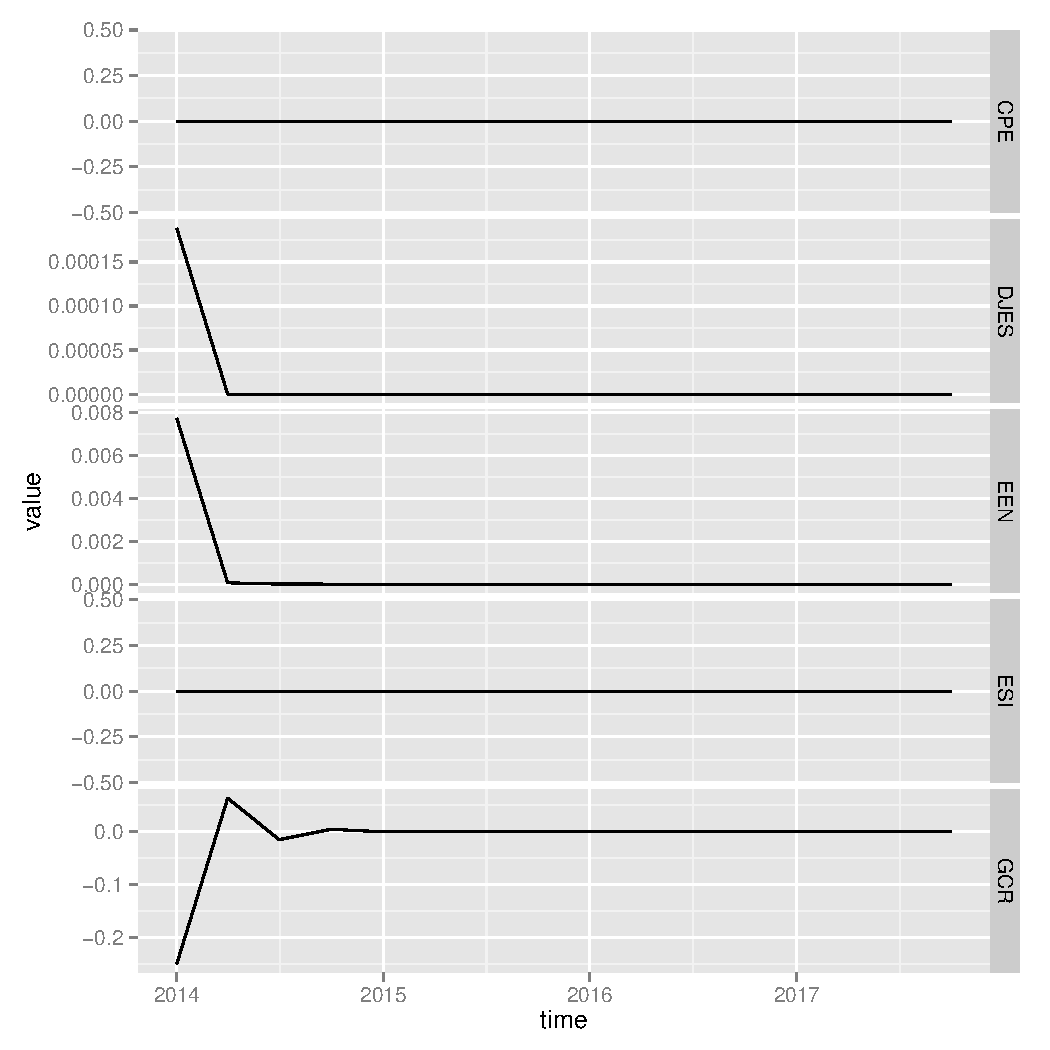
\includegraphics[width=\maxwidth]{figure/unnamed-chunk-2-1} 

\end{knitrout}


I compute the RMSE : 

\begin{knitrout}
\definecolor{shadecolor}{rgb}{0.969, 0.969, 0.969}\color{fgcolor}\begin{kframe}
\begin{alltt}
\hlstd{df2}\hlkwb{<-}\hlstd{df[}\hlnum{17}\hlopt{:}\hlnum{32}\hlstd{,]}
\hlstd{RMSE}\hlkwb{<-}\hlkwa{NULL}
\hlkwa{for} \hlstd{(i} \hlkwa{in} \hlnum{2}\hlopt{:}\hlstd{(}\hlkwd{length}\hlstd{(df)}\hlopt{-}\hlnum{1}\hlstd{))\{}
  \hlstd{RMSE[i]}\hlkwb{<-}\hlkwd{as.matrix}\hlstd{(}\hlkwd{t}\hlstd{(df2[,}\hlnum{1}\hlstd{]}\hlopt{-}\hlstd{df2[,i])}\hlopt\hlstd{(df2[,}\hlnum{1}\hlstd{]}\hlopt{-}\hlstd{df2[,i]))}\hlopt{/}\hlnum{16}
\hlstd{\}}
\hlstd{RMSEmodel}\hlkwb{<-}\hlstd{RMSE[}\hlopt{-}\hlnum{1}\hlstd{]}
\hlkwd{names}\hlstd{(RMSEmodel)}\hlkwb{<-}\hlkwd{names}\hlstd{(df[}\hlnum{2}\hlopt{:}\hlnum{10}\hlstd{])}
\end{alltt}
\end{kframe}
\end{knitrout}



% latex table generated in R 3.1.3 by xtable 1.7-4 package
% Thu Jul  9 14:38:55 2015
\begin{table}[ht]
\centering
\caption{blabla} 
\label{Test_table}
{\footnotesize
\begin{tabular}{rllr}
  \toprule 
 Model & lag & adaptive & RMSE \\
 \midrule 
       1 & 1 & non & 0.000794 \\ 
        2 & 2 & non & 0.001280 \\ 
        3 & 3 & non & 0.001330 \\ 
        4 & 1 & lasso & 0.000698 \\ 
        5 & 2 & lasso & 0.000616 \\ 
        6 & 3 & lasso & 0.000634 \\ 
        7 & 1 & ridge & 0.000184 \\ 
        8 & 2 & ridge & 0.001593 \\ 
        9 & 3 & ridge & 0.001390 \\ 
   \bottomrule 
\end{tabular}
}
\end{table}





\end{document}
